%Presentation of my thesis
\documentclass[]{beamer}
\usepackage{pgfpages}
\usepackage[utf8]{inputenc}
\usepackage[italian]{babel}
\usepackage{setspace}
\usepackage{color}
\usepackage{xcolor}
\usepackage{listings}
\usepackage{caption}
\usepackage{float}
\usepackage{hyperref} %for links in the table of contents
\hypersetup{hidelinks}
%theme of slides
\usetheme{CambridgeUS}

\pgfdeclareimage[height=1cm]{logoUnipd}{img/unipd}
\pgfdeclareimage[height=2cm]{logoDei}{img/dei}
\logo{\pgfuseimage{logoUnipd}}
 \titlegraphic{\pgfuseimage{logoDei}}

\title[Note di credito]{Sviluppo della gestione delle note di credito in un
programma di fatturazione}
\author[Davide Fontana]{Laureando: Davide Fontana \\Relatore: Ch.mo Prof.\ Carlo Ferrari }
\date[21/09/2016]{21 Settembre \\ Anno accademico 2015/2016}
\institute[DEI Unipd]{Corso di Laurea in Ingegneria Informatica\\ Department of Information Engineering}

\begin{document}

    \frame{\titlepage}

    \begin{frame}
        \frametitle{Azienda Ospitante}
        \begin{figure}[H]
            \centering
            \includegraphics[scale=0.4]{img/consoft}\label{logo:consoft}
        \end{figure}
    \end{frame}

    

    \begin{frame}
        \frametitle{Progetto Note di Credito}
        \begin{LARGE}
            Analisi dei requisiti 
        \end{LARGE}
        \newline
        \newline
        Utilizzo della nota di credito:
        \begin{itemize}
            \item Correttiva parziale.
            \item Annullamento di una fattura.
        \end{itemize}
    \end{frame}

    \begin{frame}
        \frametitle{Database: Schema concettuale}
        \begin{figure}[H]
            \centering
            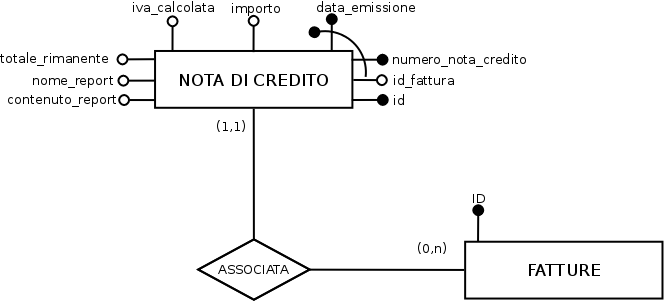
\includegraphics[scale=0.3]{img/schema_concettuale}\label{schema:concettuale}
        \end{figure}
    \end{frame}

    \begin{frame}
        \frametitle{Database: Schema logico}
        \begin{figure}[H]
            \centering
            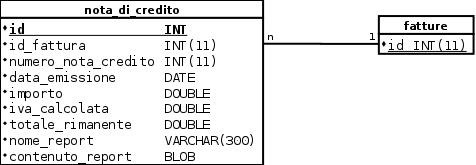
\includegraphics[scale=0.3]{img/schema_logico}\label{schema:logico}
        \end{figure}
    \end{frame}

    \begin{frame}
        \frametitle{Database: Codice SQL}
        \lstinputlisting[basicstyle=\tiny]{code/tabella.sql}
    \end{frame}

    \begin{frame}
        \begin{center}
            \Huge Parte Applicativa
        \end{center}
    \end{frame}

    \begin{frame}
            \frametitle{Tecnologie Utilizzate}
            \begin{itemize}
                \item Hibernate
                    \newline
                    Vantaggi:
                    \begin{itemize}
                        \item Tutta la gestione della connessione al database viene 
                            gestita dal framework.
                        \item Il reperimento dati viene fatto chiamando funzioni di 
                            Hibernate e non più scrivendo query. 
                        \item Tutto quello che viene restituito dalle funzioni di 
                            Hibernate sono oggetti Java.
                    \end{itemize}
                \item Spring
                    \newline
                    Vantaggi:
                    \begin{itemize}
                        \item Semplificazione sviluppo di applicativi web in Java.
                        \item Presenza di numerose estensioni.
                    \end{itemize}
            \end{itemize}
    \end{frame}

    \begin{frame}
        \frametitle{Bean delle note di credito}
        \lstinputlisting[basicstyle=\tiny,firstline=22,lastline=50]{code/bean/NotaDiCredito.java}
    \end{frame}

    \begin{frame}
        \frametitle{Lista delle fatture}
        \begin{figure}[H]
            \centering
            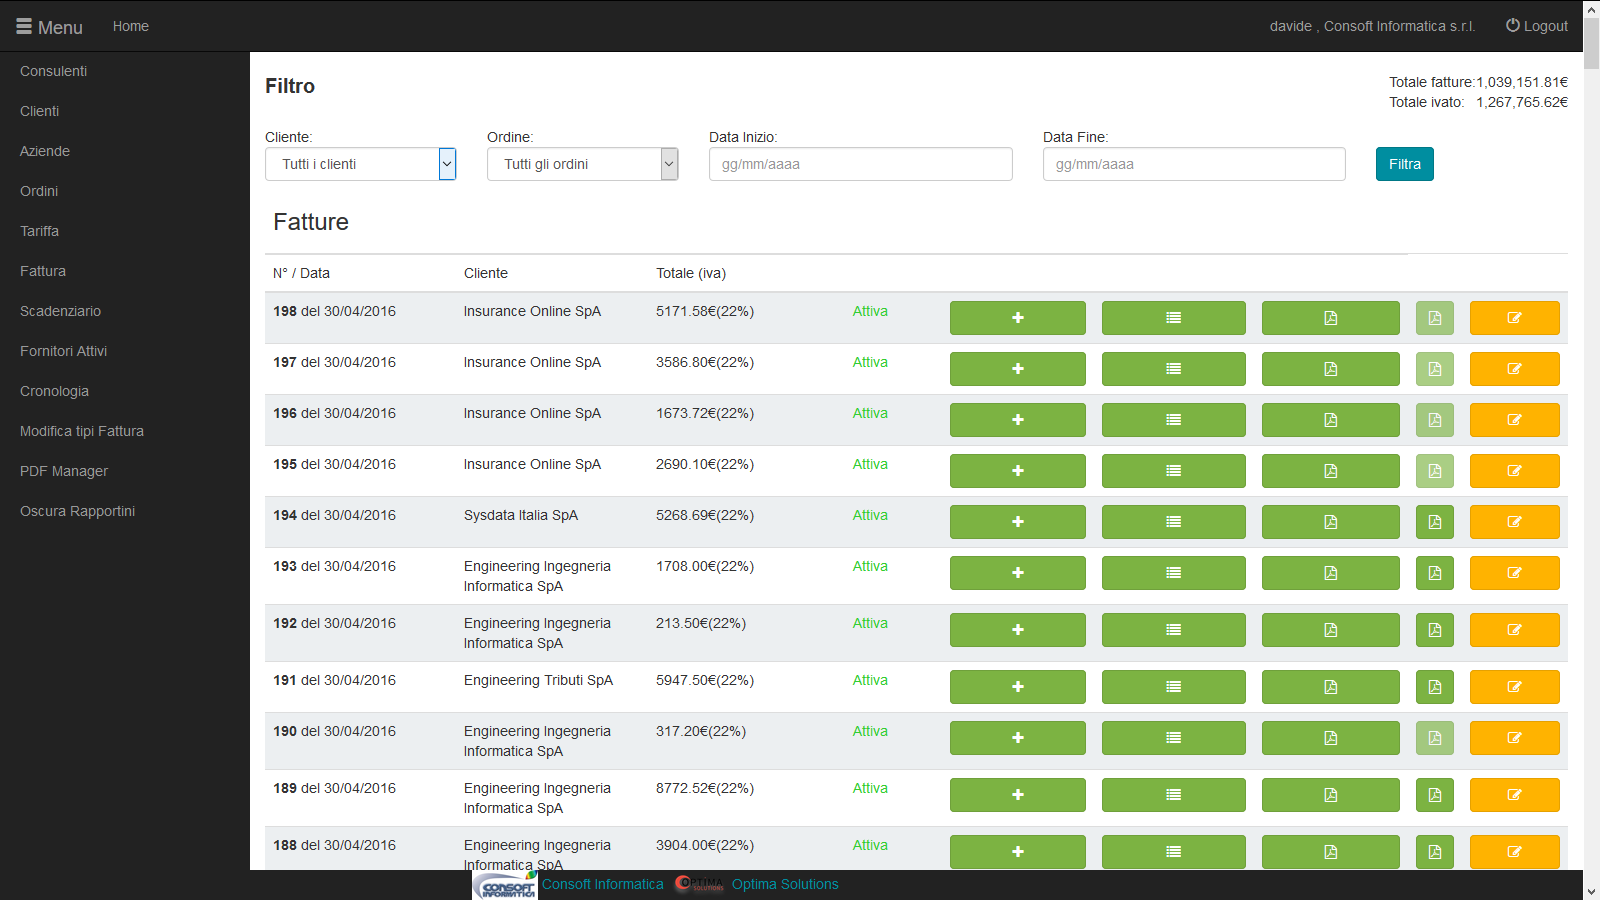
\includegraphics[scale=0.25]{img/lista_fatture}\label{img:lista_fatture}
        \end{figure}
    \end{frame}

    \begin{frame}
        \frametitle{Inserimento e modifica delle note di credito}
        \begin{figure}[H]
            \centering
            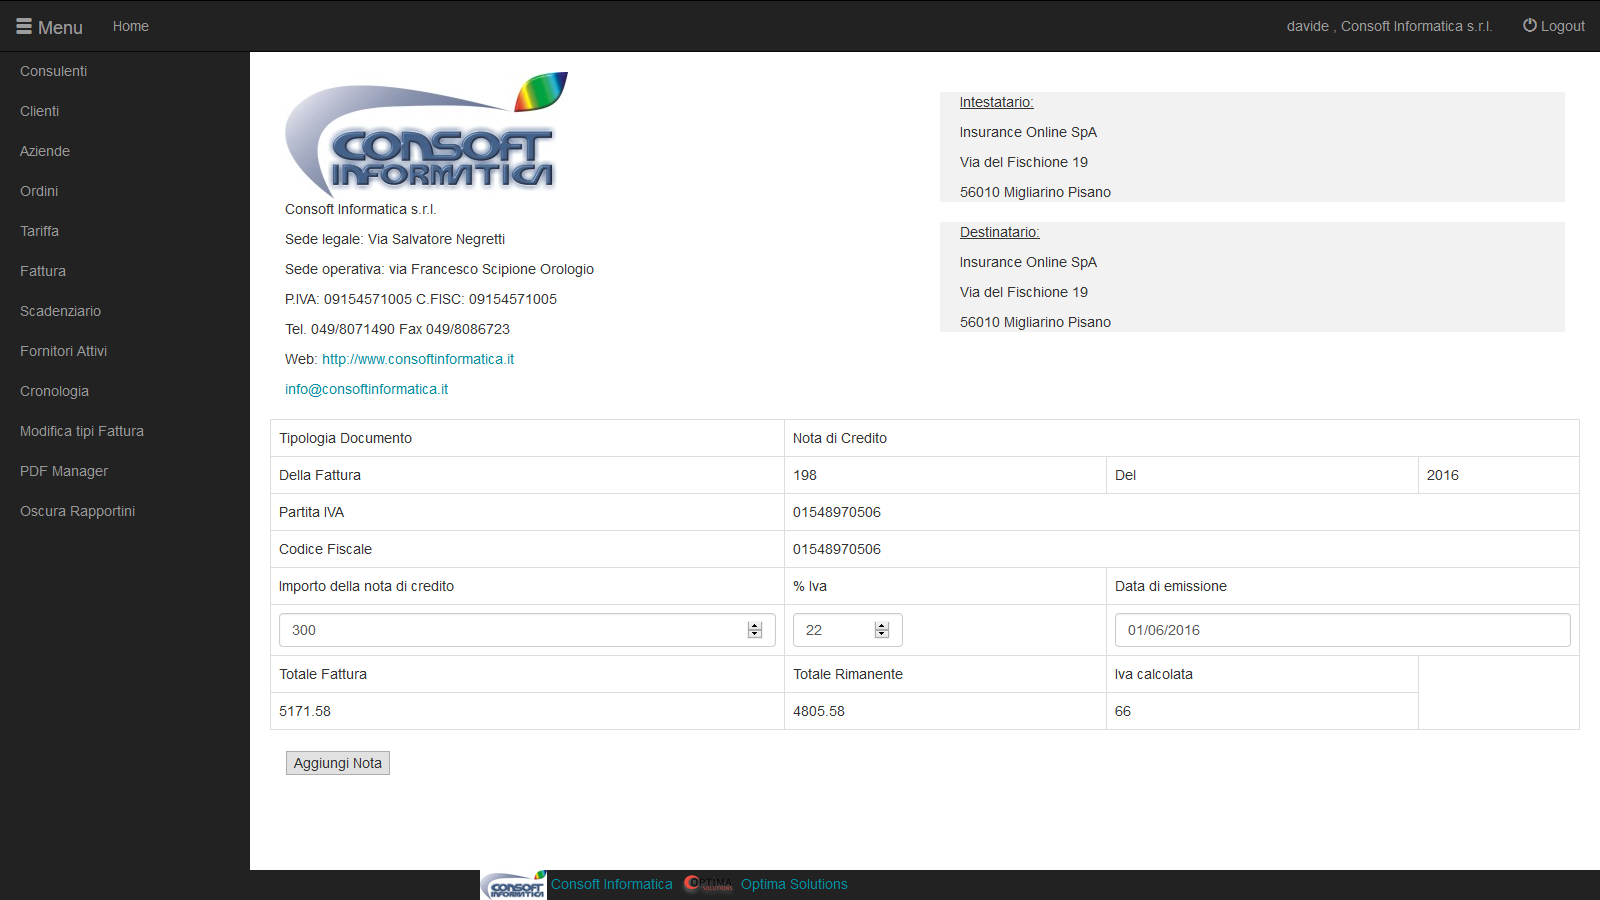
\includegraphics[scale=0.25]{img/inserimento_nota_credito}\label{fig:insert}
        \end{figure}
    \end{frame}


    \begin{frame}
        \frametitle{Pagina jsp (1)}
        \lstinputlisting[firstline=100,lastline=130,basicstyle=\ttfamily\tiny]{code/view/inserimentoModificaNoteCredito.jsp}
    \end{frame}


    \begin{frame}
        \frametitle{Pagina jsp (2)}
        \lstinputlisting[firstline=130,lastline=158,basicstyle=\ttfamily\tiny]{code/view/inserimentoModificaNoteCredito.jsp}
    \end{frame}

    \begin{frame}
        \frametitle{Form di validazione}
        \lstinputlisting[firstline=16,lastline=33,basicstyle=\ttfamily\tiny]{code/form/NotaCreditoForm.java}
    \end{frame}

    \begin{frame}
        \frametitle{Pagina jsp (3)}
        \lstinputlisting[firstline=159,lastline=172,basicstyle=\ttfamily\tiny]{code/view/inserimentoModificaNoteCredito.jsp}
    \end{frame}

    \begin{frame}
        \frametitle{Codice Javascript Front-End}
        \lstinputlisting[firstline=175,lastline=190,basicstyle=\ttfamily\tiny]{code/view/inserimentoModificaNoteCredito.jsp}
    \end{frame}

    \begin{frame}
        \frametitle{Controller: Controllo dei dati inseriti}
        \lstinputlisting[firstline=269,lastline=285,breaklines=True,basicstyle=\ttfamily\tiny]{code/controller/NotaCreditoController.java}
    \end{frame}

    \begin{frame}
        \frametitle{Controller: Salvataggio dei dati e generazione del pdf}
        \lstinputlisting[firstline=332,lastline=344,breaklines=True,basicstyle=\ttfamily\tiny]{code/controller/NotaCreditoController.java}
    \end{frame}

    \begin{frame}
        \frametitle{Controller: Caricamento dati nella fase di modifica}
        \lstinputlisting[firstline=192,lastline=214,breaklines=True,basicstyle=\ttfamily\tiny]{code/controller/NotaCreditoController.java}
    \end{frame}

    \begin{frame}
        \frametitle{Lista delle Note di Credito}
        \begin{figure}[H]
            \centering
            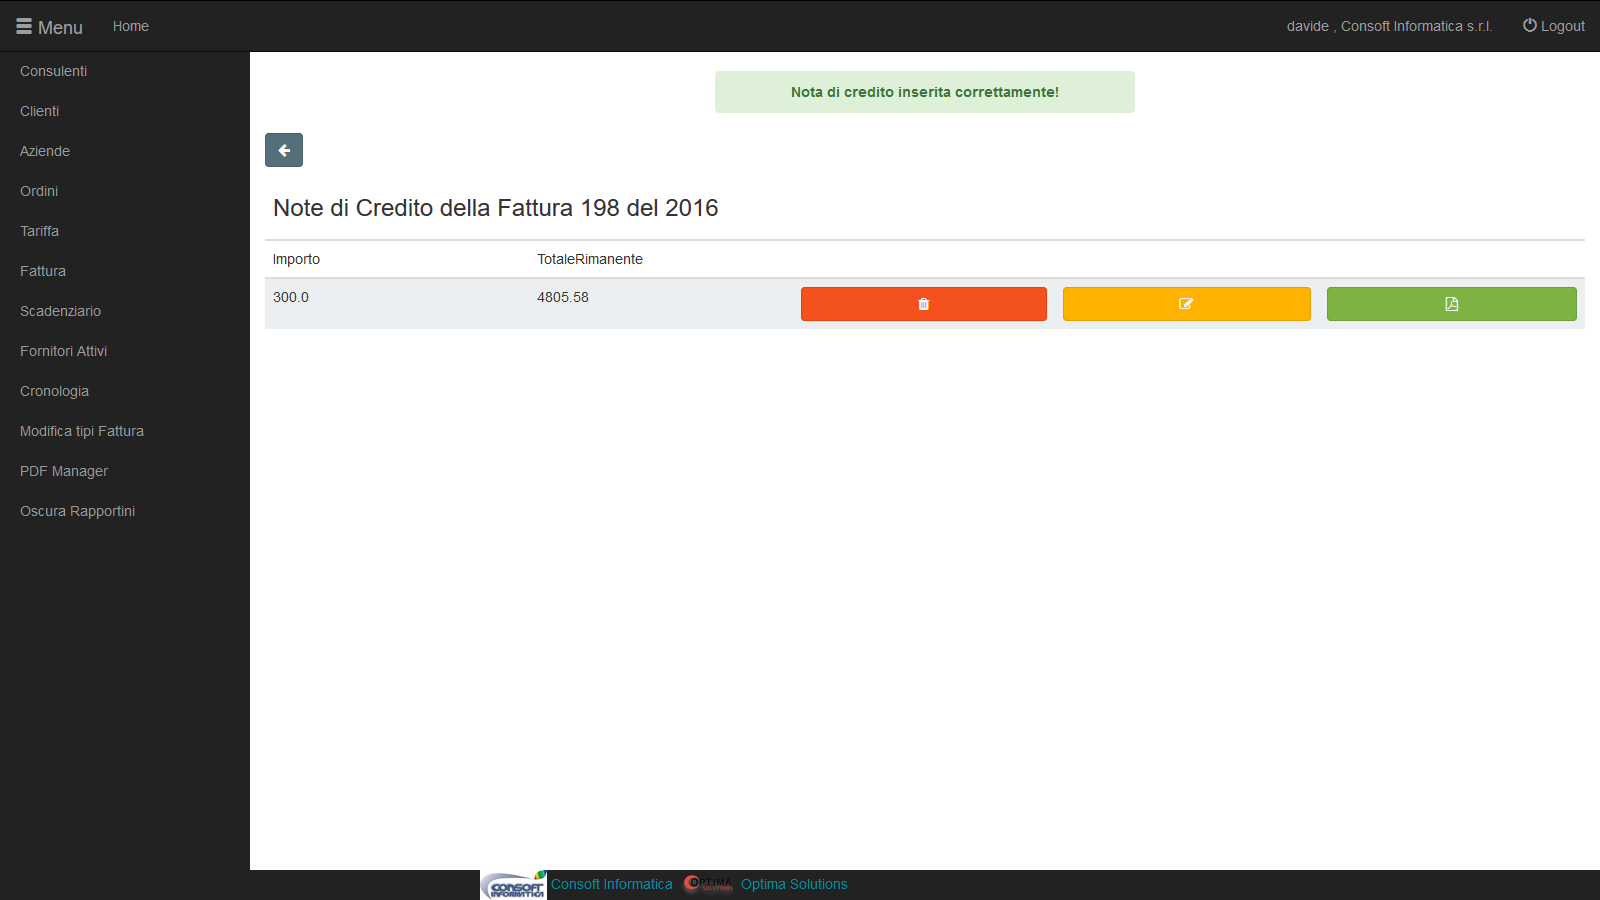
\includegraphics[scale=0.25]{img/visualizzazione_note_credito}\label{fig:visualizzazione}
        \end{figure}
    \end{frame}

    \begin{frame}
        \frametitle{Controller: Ritorno delle Note di Credito}
        \lstinputlisting[firstline=90,lastline=112,breaklines=True,basicstyle=\ttfamily\tiny]{code/controller/NotaCreditoController.java}
    \end{frame}

    \begin{frame}
        \frametitle{Controller: Visualizzazione del pdf}
        \lstinputlisting[firstline=535,lastline=550,breaklines=True,basicstyle=\ttfamily\tiny]{code/controller/NotaCreditoController.java}
    \end{frame}

    \begin{frame}
        \frametitle{Risultato finale}
        \begin{figure}[H]
            \includegraphics[scale=0.25]{pdf/nota}\label{fig:nota}
        \end{figure}
    \end{frame}

    \begin{frame}
        \begin{center}          
            \huge Conclusioni
        \end{center}
    \end{frame}

    \begin{frame}
        \begin{center}
            \huge Slide di approfondimento. 
        \end{center}
    \end{frame}

    \begin{frame}
        \frametitle{Spring MVC}
        \begin{figure}[H]
            \centering
            \includegraphics[scale=0.3]{img/spring_mvc_structure}\label{spring:diagram}
        \end{figure}
    \end{frame}

    \begin{frame}
        \frametitle{Codice di decisione per la variabile \(\texttt{\$\{azione\}}\)}
        \lstinputlisting[firstline=8,lastline=14,basicstyle=\ttfamily\tiny]{code/view/inserimentoModificaNoteCredito.jsp}
    \end{frame}
\end{document}

